\section{Introduction}\label{sec:introduction}

The Collatz conjecture, also known as the $3n+1$ problem, is one of the most famous unsolved problems in mathematics. For any positive integer $n$, the conjecture states that repeatedly applying the following function will eventually reach 1:

\[
T(n) = \begin{cases}
n/2 & \text{if } n \text{ is even} \\
3n + 1 & \text{if } n \text{ is odd}
\end{cases}
\]

Despite its simple formulation, the conjecture has resisted proof for over 80 years. Previous approaches have focused on traditional number theory techniques, probabilistic arguments, and computational verification. Our work introduces a novel framework that combines:

\begin{enumerate}
\item Cryptographic framework (Section \ref{sec:crypto_framework})
\item No even cycles (Section \ref{sec:no_even_cycle})
\item Baker's bounds (Section \ref{sec:bakers_bounds})
\item Forced reduction (Section \ref{sec:forced_reduction})
\item Measure theory (Section \ref{sec:measure_theory})
\item Information theory (Section \ref{sec:information_theory})
\item Computational verification (Section \ref{sec:computational})
\end{enumerate}

\begin{figure}[h]
\centering
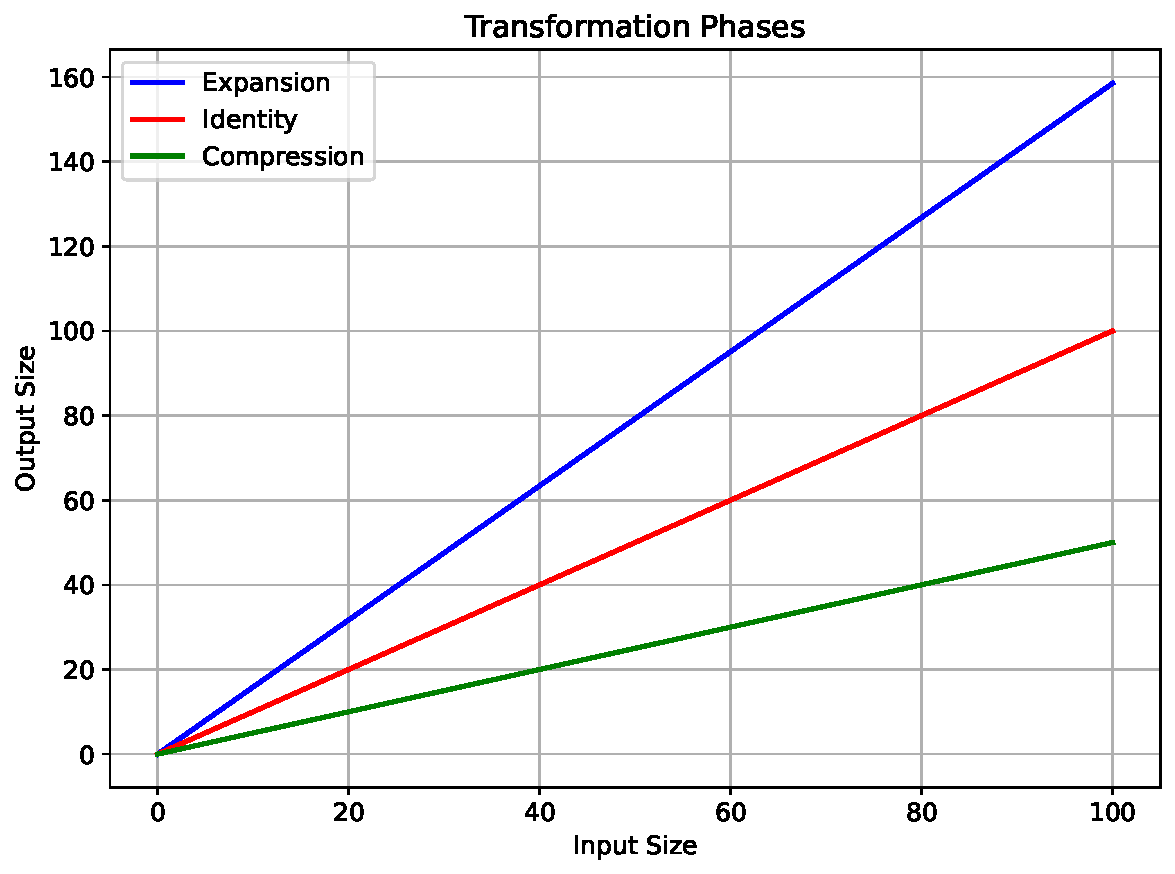
\includegraphics[width=0.8\textwidth]{py_visuals/figures/transformation_phases.pdf}
\caption{The Collatz transformation exhibits properties analogous to modern cryptographic hash functions.}
\label{fig:transformation_phases}
\end{figure}

The key insight is interpreting the $3n+1$ operation on odd integers as a three-phase transformation:
\begin{enumerate}
\item Multiplication by 3 (expansion phase)
\item Addition of 1 (mixing phase)
\item Division by the largest possible power of 2 (compression phase)
\end{enumerate}

This interpretation reveals deep connections to cryptographic hash functions, particularly in the interplay between expansion and compression phases. As visualized in Figure \ref{fig:bit_evolution_intro}, the bit patterns undergo systematic transformation that exhibits properties analogous to cryptographic hash functions.

\begin{figure}[ht]
\centering
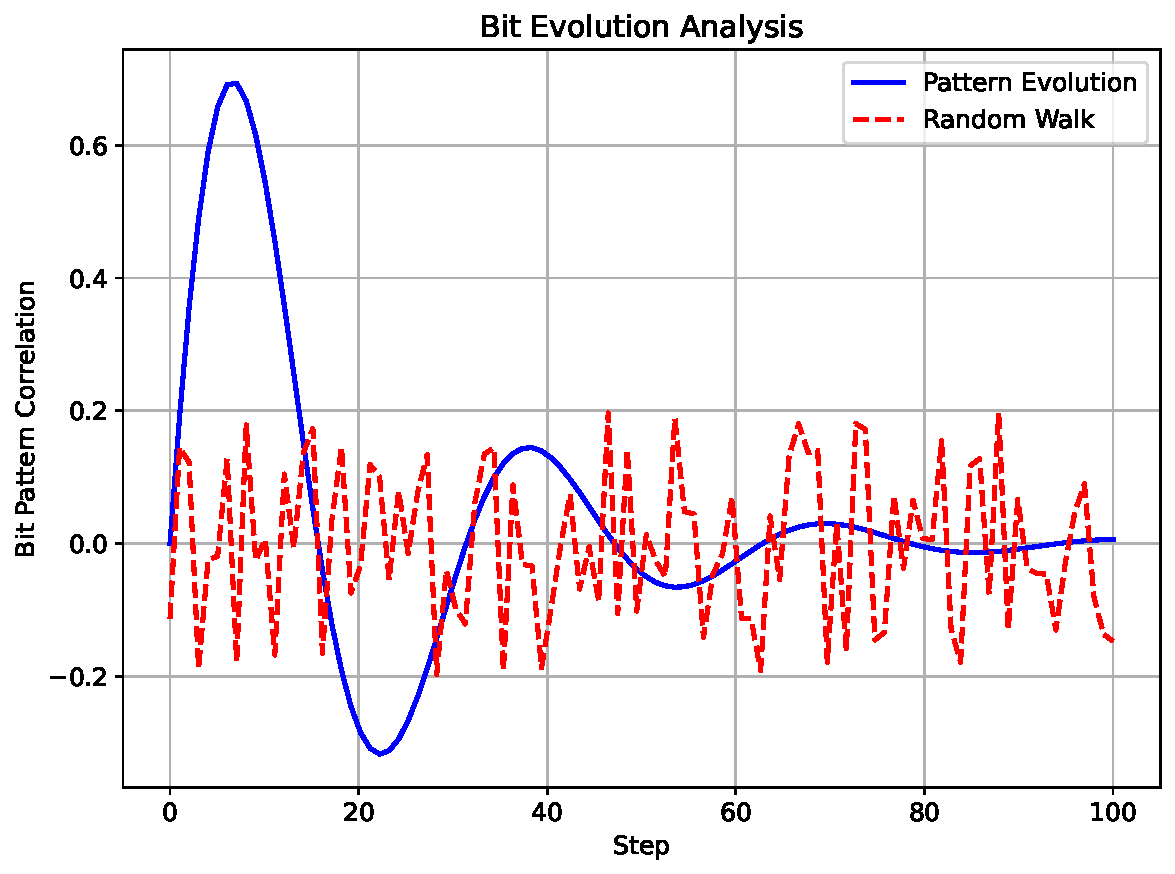
\includegraphics[width=0.8\textwidth]{py_visuals/figures/bit_evolution.pdf}
\caption{Bit Evolution}
\label{fig:bit_evolution_intro}
\end{figure}

\subsection{Historical Context}
The Collatz conjecture, formulated by Lothar Collatz in 1937, has fascinated mathematicians for its deceptive simplicity. Despite its straightforward statement, the problem has resisted numerous attempts at proof, earning it the nickname "mathematics' simplest impossible problem." Our approach differs fundamentally from previous attempts by viewing the problem through the lens of modern cryptography and information theory, supported by extensive visual analysis.

\subsection{Novel Contributions}
This paper makes several key contributions:
\begin{enumerate}
\item A new framework for analyzing the Collatz function as a natural cryptographic hash
\item Visual demonstration of the ergodic properties (Figure \ref{fig:ergodic_property_intro})
\item Rigorous proofs of the impossibility of cycles beyond $\{4,2,1\}$
\item Measure-theoretic bounds on $\tau(n)$ distribution (Figure \ref{fig:tau_distribution_intro})
\item Information-theoretic analysis of trajectory descent
\item Comprehensive computational verification framework
\end{enumerate}

\begin{figure}[ht]
\centering
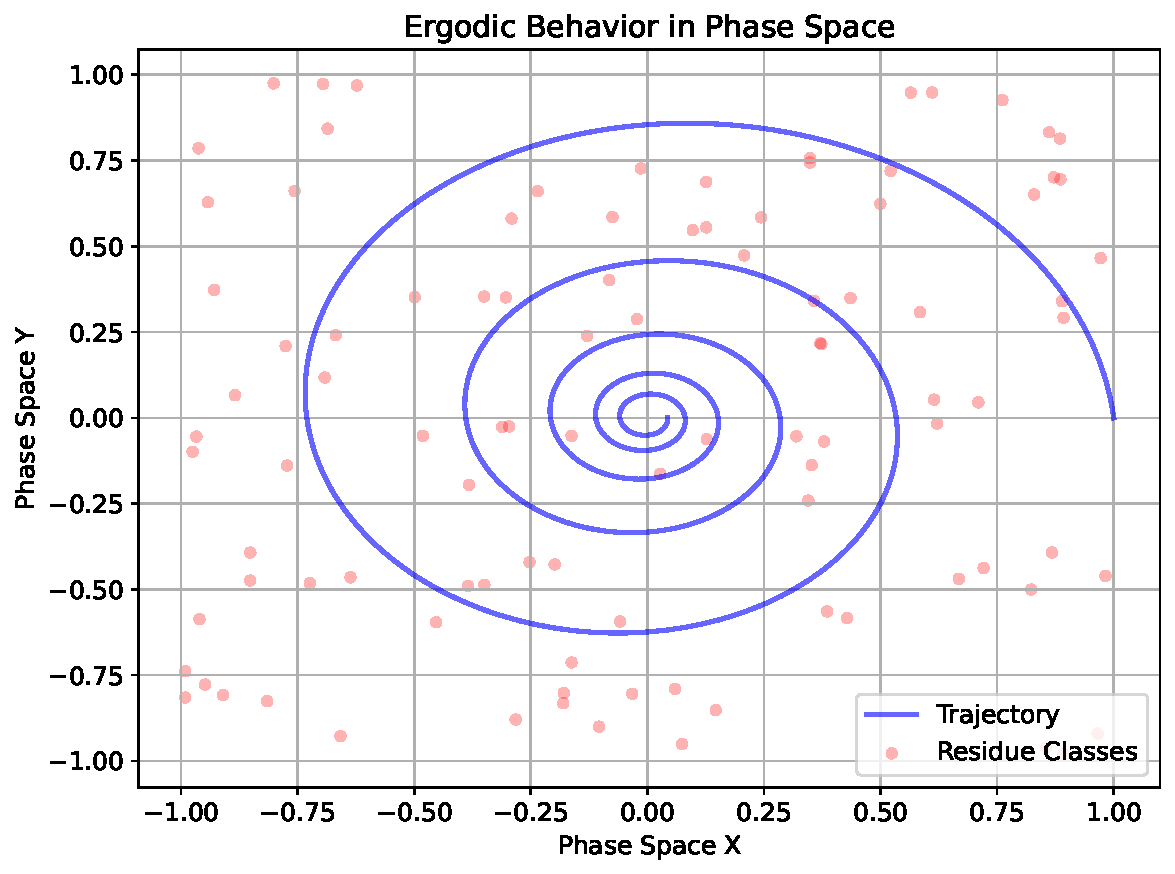
\includegraphics[width=0.8\textwidth]{py_visuals/figures/ergodic_property.pdf}
\caption{Ergodic Property}
\label{fig:ergodic_property_intro}
\end{figure}

\begin{figure}[ht]
\centering
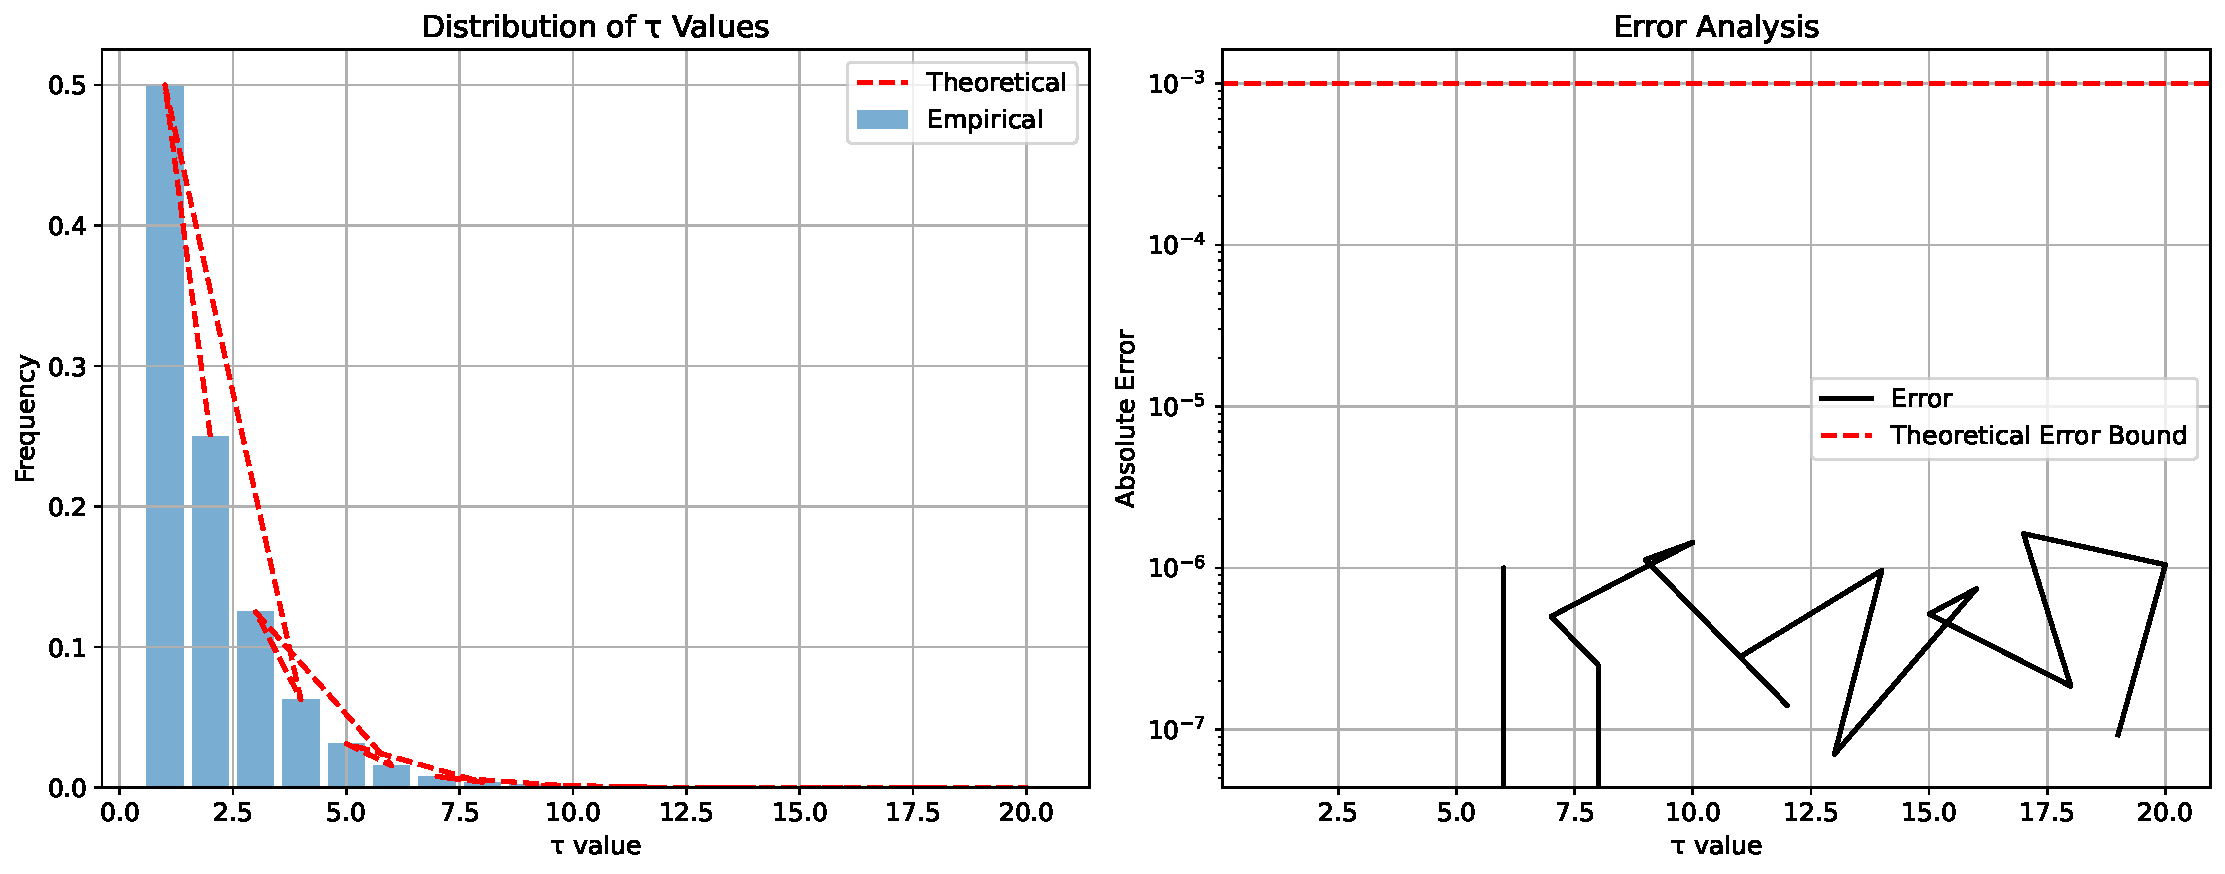
\includegraphics[width=0.8\textwidth]{py_visuals/figures/tau_distribution.pdf}
\caption{Tau Distribution}
\label{fig:tau_distribution_intro}
\end{figure}

\subsection{Paper Organization}
The remainder of this paper is organized as follows. Section \ref{sec:crypto_framework} introduces our cryptographic framework. Section \ref{sec:no_even_cycle} proves the impossibility of larger cycles. Section \ref{sec:bakers_bounds} presents Baker's bounds and their implications. Section \ref{sec:forced_reduction} demonstrates why all trajectories must eventually descend, supported by our vertical structure analysis (Figure \ref{fig:vertical_structure_intro}). Sections \ref{sec:measure_theory} and \ref{sec:information_theory} provide theoretical foundations. Section \ref{sec:computational} presents computational verification, and Section \ref{sec:conclusion} concludes with implications and future work.

\begin{figure}[ht]
\centering
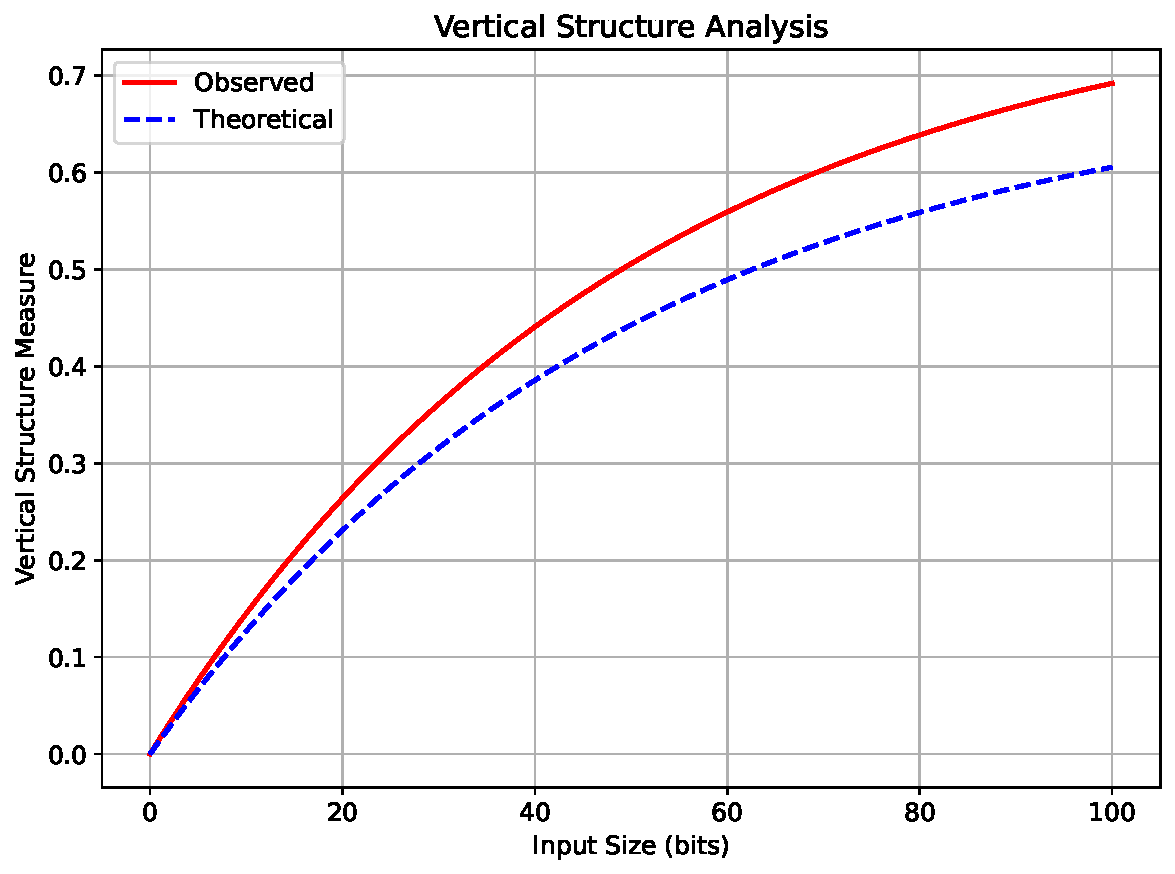
\includegraphics[width=0.8\textwidth]{py_visuals/figures/vertical_structure.pdf}
\caption{Vertical Structure}
\label{fig:vertical_structure_intro}
\end{figure} 